% ===================================================
% CHAPITRE 9 — ARCIS
% Pages imprimées 47-50 — vues 50-53
% ===================================================
\chapter{Arcis}

% --- Page imprimée 47 — vue 50
\begin{figure}[htbp]
    \centering
    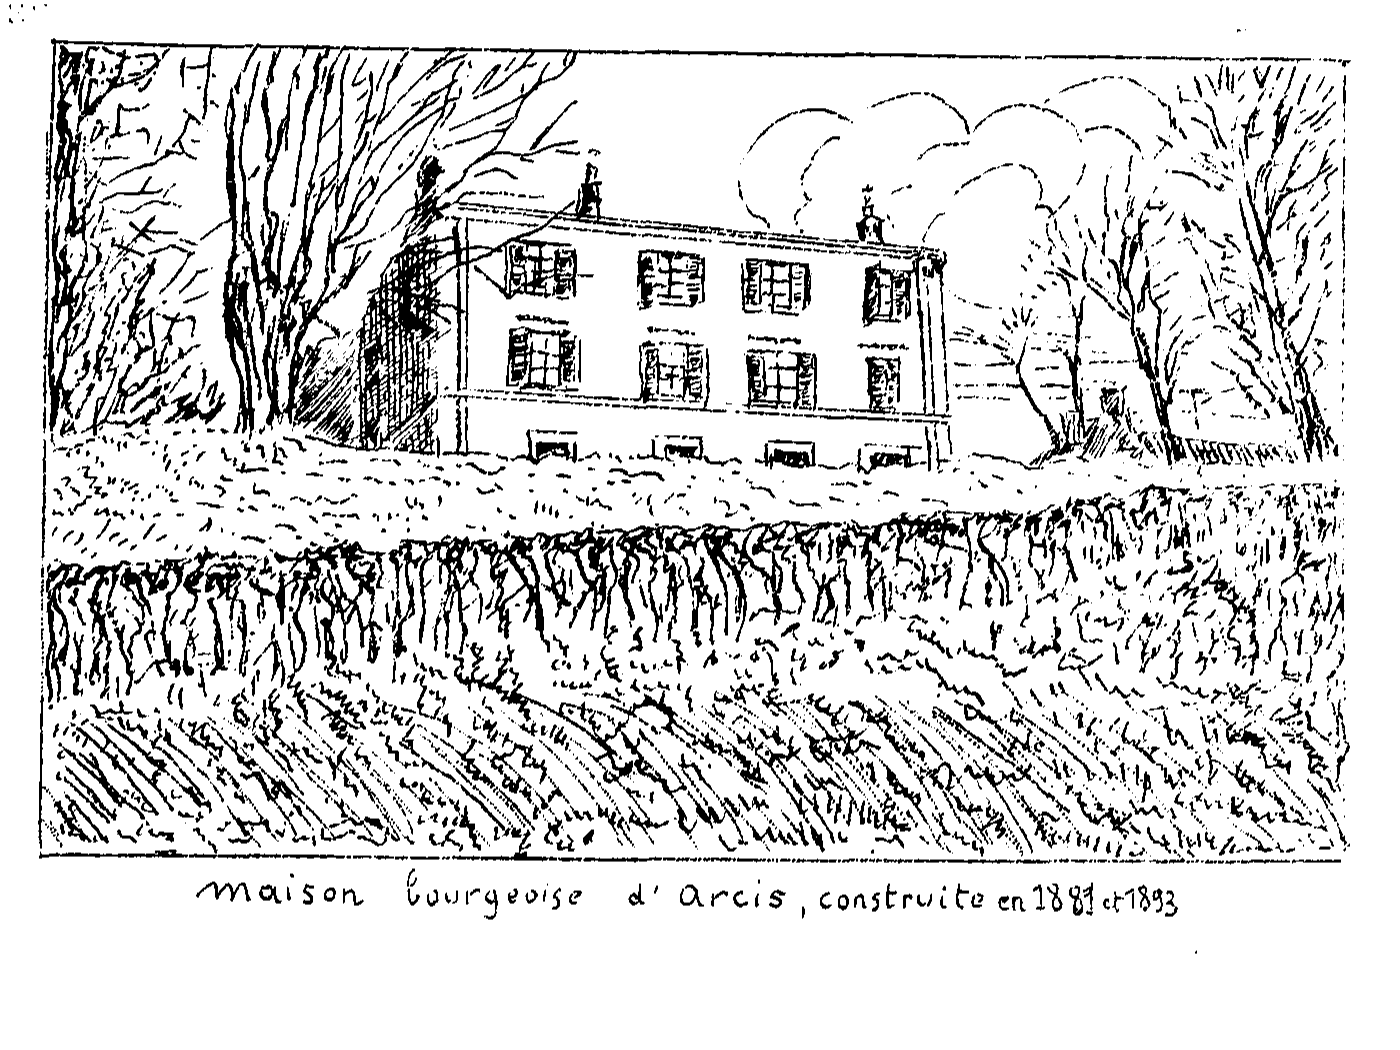
\includegraphics[width=0.72\textwidth]{Illustrations/illus-arcis-maison.png}
    \caption*{Maison bourgeoise d'Arcis, construite en 1881 et 1893}
\end{figure}

Le nom latin d'Arcis qui signifie Citadelle réveille en nous l'idée d'une maison forte, d'un de ces manoirs rendus nécessaires par les luttes incessantes du moyen-âge et que les Seigneurs élevaient sur nos montagnes pour faire respecter leurs droits par leurs ennemis, souvent même par leurs suzerains. Arcis a pu faire partie d'un système de défense ; organisé à une époque fort reculée, pour protéger la vallée de la Grosne et par là même la partie méridionale du Mâconnais. Indépendamment de Nagu qui commandait la vallée proprement dite, Alloignet surveillait les communications qui avaient lieu, depuis la fondation de Beaujeu par la vallée de Lacarelle, comme Arcis était la clef de la partie orientale du Beaujolais.

% --- Page imprimée 48 — vue 51
Le château était construit sur les flancs de la montagne qui domine, au levant, la vallée des Jambons. Son existence nous est attestée par des ruines disparues aujourd'hui, mais qui existaient encore au commencement du siècle dernier. Dans des travaux exécutés récemment (vers 1850), on a mis à jour des murs épais et d'une solidité à toute épreuve ; Monsieur Moretain signale même des traces évidentes de fossés comblés dans la suite, avec les débris des remparts.

D'ailleurs, comme à Ouroux, dans toutes les fouilles que les constructions nouvelles ont nécessitées, on a pu constater la présence de cendres et de bois à demi-consumés, preuve qu'Arcis fut incendié à une époque qu'aucun document ne permet de préciser. Il semble que nous pouvons admettre pour Arcis les mêmes causes de destruction que pour Nagu. Les Tard-Venus ou les Routiers seraient encore ici les auteurs de l'incendie et partant de la disparition du château.

Relevé bientôt de ses ruines, il conserva son nom primitif sans offrir néanmoins les caractères de maison forte proprement dite. Nous n'avons, il est vrai, aucune preuve de ce fait ; mais après le désastre dont il fut victime vers la fin du XIVe siècle, Ouroux ne joua plus qu'un rôle tout-à-fait secondaire dans la province et l'histoire nous eût conservé la date et les causes du démantèlement d'Arcis, si le château eût été fortifié de nouveau. Tout porte à croire que l'on utilisa, dans les nouvelles constructions les parties du bâtiment restées debout ; d'ailleurs les découvertes successivement opérées montrent bien que les maisons plus récentes ont été élevées en dehors de l'enceinte primitive.

Quels furent les premiers possesseurs du fief d'Arcis ? Nous devons ici nous contenter des auteurs qui ont écrit sur le Beaujolais. Les renseignements qu'ils nous donnent sont de plus très incomplets et peu précis. Ainsi l'Album Lyonnais nous a conservé les noms de Nanton qui possédait Arcis en 1342 et celui de Henri de Pizeys en 1374.

Henri de Pizeys appartenait à une noble et puissante famille qui portait le nom du fief de Pizeys situé sur la paroisse de St Jean d'Ardières.

% --- Page imprimée 49 — vue 52
% La page originale juxtapose le panneau héraldique à gauche et le
% texte courant à droite. Les cinq entrées sont volontairement composées
% en petites unités pour conserver cette lecture et cette hiérarchie.
\newcommand{\arcisblason}[3]{%
    \noindent
    \begin{minipage}[t]{0.49\linewidth}
        \vspace{0pt}\centering
        \includegraphics[width=\linewidth]{#1}%
    \end{minipage}%
    \hfill
    \begin{minipage}[t]{0.47\linewidth}
        \vspace{0pt}\scriptsize\raggedright\setlength{\parskip}{0pt}
        #2\\[-0.1ex]
        #3
    \end{minipage}\par\medskip
}%
\clearpage
\noindent
\begin{minipage}[t]{0.43\textwidth}
    \vspace{0pt}
    \begin{center}\textsc{Armes des}\end{center}
    \setlength{\parskip}{0pt}
    \arcisblason{Illustrations/illus-arcis-armoiries-nanton.png}{De Nanton}{Seigneur de Pizey\\De sinople\\à la croix d'or.}
    \arcisblason{Illustrations/illus-arcis-armoiries-pizeys.png}{De Piseys}{D'argent\\au chef bandé d'or et d'azur\\de 6 pièces}
    \arcisblason{Illustrations/illus-arcis-armoiries-madelaine.png}{De La Madelaine-Ragny}{Seigneur de Corcelles\\Écartelé au 1 d'hermine\\à 3 bandes de gueules,\\chargées de 9 coquilles d'or.\\2, 5 et 2 ;\\au 2, d'or, à la croix\\ancrée de gueules ;\\au 3 de gueules, à\\3 bandes d'argent ;\\au 4 d'or et d'azur,\\de 6 pièces ;\\à la bordure de gueules\\Devise :\\Posita Feritate nitescit}
    \arcisblason{Illustrations/illus-arcis-armoiries-tircuy.png}{Tircuy de Corcelles}{Seigneur de Corcelles, d'Arcis\\de Flourye\\D'azur, à la fasce d'or}
    \arcisblason{Illustrations/illus-arcis-armoiries-bottu.png}{Bottu de la Barmondière}{Seigneur de Montgré\\D'azur, au chevron d'or\\accompagné en pointe\\d'un lion du même,\\au chef d'or.}
\end{minipage}%
\hfill
\begin{minipage}[t]{0.54\textwidth}
    \vspace{0pt}\fontsize{12}{16.2}\selectfont\ttfamily\raggedright
    Le fief d'Arcis passa, au siècle suivant, à la famille de Nagu-Varennes. On sait que Pierre Nagu le possédait en 1463.

    Le 1er Mars 1539, noble Gérard de la Maddeleine-Ragny donna à son tour le dénombrement de ce fief.

    Vers la fin du XVIe siècle, Arcis fut vendu à un gentilhomme bourguignon, noble Lazare de Tircuy de la Barre, écuyer, qui en fournit le dénombrement le 2 Juillet 1601.

    Un acte de vente nous signale un nouveau propriétaire. Par contrat passé en 1659, messire Louis Damarin du Rousset, écuyer, seigneur de Corcelles et d'Arcis achetait le domaine dit de Métrat, aujourd'hui Fontmartin, paroisse de Vauxrenard, d'Antoine de Lafont. Un extrait des rôles pour les étapes nous le signale comme possédant deux domaines sur Ouroux en 1661.

    Vers la fin du même siècle, Arcis fut acquis par François de la Barmondière dont la famille originaire d'Auvergne remontait à une haute antiquité. Il fit de 1706 à 1713 de nombreuses réparations dans ses domaines d'Arcis, des Mélinands et de Mettrat. Son représentant à Ouroux à cette époque était Monsieur Duligier Testenoire. Nous n'avons aucun détail sur lui et le nom de son successeur ne nous a pas été conservé. Son petit fils fut François Louis de la Barmondière, seigneur de Montgré, Arcis et
\end{minipage}
\clearpage
% --- Page imprimée 50 — vue 53 (suite)
autres lieux. Il fut fait prisonnier pendant la grande Révolution et guillotiné. Il laissa une fille unique morte sans alliance. Celle-ci céda ses biens à Monsieur de Verna qui vendit Arcis à Monsieur Berloty, notaire à Lyon. Actuellement Arcis appartient aux deux familles Boffard-Berloty, Rambaud-Berloty et à leurs descendants.

Dès 1686, le Seigneur d'Arcis avait droit de justice sur une partie de la paroisse. Sa juridiction s'étendait sur toute la partie qui est à l'orient de la Grosne. Ainsi la ferme Daguin appartenant au Seigneur de St-Julien dépendait de la justice d'Arcis comme nous le prouve un jugement porté en 1703. En 1686 Philibert de Lafont était procureur et Jean Gobet juge de la Seigneurerie.

Par suite de quelles circonstances Arcis devint-il le siège d'une justice ? Le voici : En 1532, François Ier ayant besoin de se créer de nouvelles ressources pour soutenir sa lutte contre Charles-Quint, nomma des commissaires chargés de vendre le domaine de la Baronnie de Beaujeu. Les seigneuries, les justices, les péages, les greffes, tout fut converti en argent mais toutefois sous condition de rachat. En 1538, Louis de Bourbon, neveu et héritier du Connétable ayant été remis en possession de la Seigneurerie, racheta à ses frais, les aliénations qui avaient été faites.

En 1600, Henri de Bourbon Montpensier recommença de nouveau à mettre aux enchères les justices du Beaujolais. C'est de ce nombre étonnant d'aliénations, de dénombrements poussés jusqu'aux moindres divisions, continués pendant un siècle et demi, qu'est sorti cette effrayante quantité de hautes justices parmi nous. Chaque Seigneur devenant justicier créa une sorte de tribunal informe dont les offices étaient remplis par des gens sans instruction, sans habitude des affaires. Nos villages virent s'établir cette foule de praticiens, qui dans la même heure remplissaient les fonctions de notaire, de juge, de premier en ordre, de greffier et même d'huissier.

Nous avons cité, dans notre région, Arcis ayant droit de justice, sur une partie de la paroisse d'Ouroux et Gorze sur l'autre partie. La justice d'Avenas appartenait au Seigneur de Sauzey, celle de Vauxrenard à celui du Thil. Cet état de choses dura jusqu'à la Grande Révolution.
